\documentclass[a4paper]{article}
\usepackage{amsmath}
\usepackage{amsfonts}
\usepackage{amsthm}
\usepackage{amssymb}
\usepackage[english]{babel}
\usepackage{float}
\usepackage{graphicx}
\usepackage{hyperref}
\usepackage[utf8]{inputenc}
\usepackage{listings}
\usepackage{xcolor}
%% \usepackage{subfigure}
\usepackage{graphicx}
\usepackage{subcaption}
\usepackage{stmaryrd}

\usepackage{a4wide}
\usepackage{url}
%% \usepackage[left=2cm,top=2cm,bottom=1.5cm,right=2cm]{geometry}

\lstset{
  frame=tb,
  language=Python,
  aboveskip=3mm,
  belowskip=3mm,
  showstringspaces=false,
  formfeed=newpage,
  tabsize=4,
  comment=[l]{\#},
  breaklines=true,
  morekeywords={models, lambda, forms}
}

\newcommand{\prob}[1]{\mathbb{P}\left(#1\right)}
\newcommand{\expect}[1]{\mathbb{E}\left(#1\right)}
\newcommand{\avg}[1]{\sum_{i=1}^{#1}X_i}
\newcommand*{\QEDA}{\hfill\ensuremath{\blacksquare}}%

\title{\vspace{-5cm} Numerical Optimization \\ Individual Handin 1}
\author{Dmitry Serykh (qwl888)}

\begin{document}
\maketitle
\section*{Introduction}
I had to retake this course due to some personal reasons.
Hence, some of the solutions in this submission are based on my solutions from
the previous year. Furthermore, in the report, I reduce the problems to two
dimensions. However, my implementation of all, but Rosenbrock function support
arbitrary values of $d$.

\section{Ellipsoid Function}
\label{sec:ellipse}
The Ellipsoid function is given by:
\[
f_{1}(x)=\sum_{i=1}^{d} \alpha^{\frac{i-1}{d-1}} x_{i}^{2}, \alpha=1000
\]
The plots for the function can be seen on Figure \ref{plt1}.
\begin{figure}[H]
  \centering
  \begin{subfigure}[b]{0.49\textwidth}
    \centering
    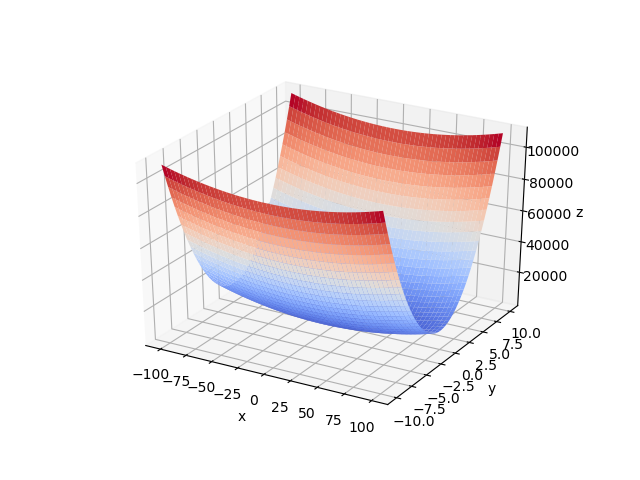
\includegraphics[width=\textwidth]{imgs/plt11}
    \caption{Surface plot}
  \end{subfigure}
  \begin{subfigure}[b]{0.49\textwidth}
    \centering
    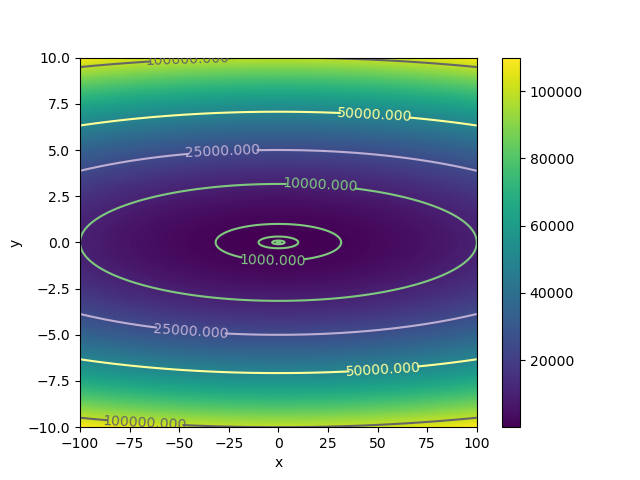
\includegraphics[width=\textwidth]{imgs/plt12}
    \caption{Contour plot}
  \end{subfigure}
  \caption{Ellipsoid Function}
  \label{plt1}
\end{figure}

\subsection{First Derivative}
I find the gradient:
\[
\nabla f_1(x_1,x_2) = 
\begin{bmatrix}
    2 x_1\\
    2\alpha x_2\\
\end{bmatrix}
\]
\subsection{Second Derivative}
Then I find the Hessian matrix, but first I will consider the function:
\[
f(x)=\sum_{i=1}^{N} g_{i}\left(x_{i}\right)
\]
$\frac{\partial g_{i}(x_{i})}{\partial x_j} = 0\text{ for }j\neq i$, since
$g_i(x_i)$ is not dependent on any $x_j$, where $j \neq i$.
And since $\frac{\partial 0}{\partial x} = 0\text{, for all }$ $x \in
\mathbb{R}^{N}$, the hessian matrix would only have nonzero values in the
entries where $j=i$. Therefore we have that the Hessian is a diagonal matrix with 
\[
(H f(x))_{i  i}=g_{i}^{\prime \prime}\left(x_{i}\right)
\]
I then use this notion in order to determine the Hessian:
\[
H(x_1, x_2) = 
\begin{bmatrix}
    2 & 0     \\
    0 & 2\alpha
\end{bmatrix}
\]

\subsection{Finding a Minimizer}
I can then solve a system of equations in order to find the stationary points:
\begin{align*}
\begin{bmatrix}
    2 x_1 \\
    2\alpha x_2 \\
\end{bmatrix}
&=
\begin{bmatrix}
    0 \\
    0    
\end{bmatrix}\\
\begin{bmatrix}
    x_1 \\
    x_2 \\
\end{bmatrix}
&=
\begin{bmatrix}
    0 \\
    0 \\
\end{bmatrix}
\end{align*}
The system of equations has only one solution, hence $(0,0)^T$ is the only
stationary point. I then determine the type of the stationary point by 
finding the determinant of the hessian matrix:

\[
det(H(0,0)) = 
det\left(\begin{bmatrix}
    2 & 0     \\
    0 & 2000
\end{bmatrix}\right)
= 4000 > 0
\]
Determinant is positive, hence I conclude that
$H(1,1)$ is positive definite, and $(0,0)^T$ is the only local minimizer of the
Ellipsoid function.


\section{Rosenbrock Function}
\label{sec:rosenbrock}
The Rosenbrock function is given by:
\[
f_2(x_1,x_2) = 100(x_2 - x_1^2)^2 + (1 - x_1)^2
\]
The plots for the function can be seen on Figure \ref{plt2}.
\begin{figure}[H]
  \centering
  \begin{subfigure}[b]{0.49\textwidth}
    \centering
    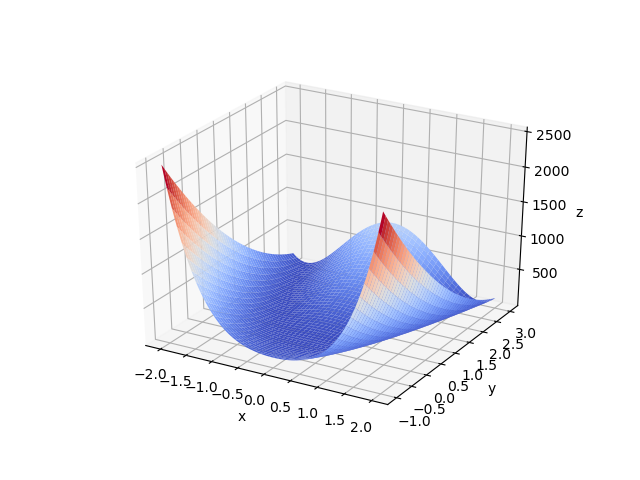
\includegraphics[width=\textwidth]{imgs/plt21}
    \caption{Surface plot}
  \end{subfigure}
  \begin{subfigure}[b]{0.49\textwidth}
    \centering
    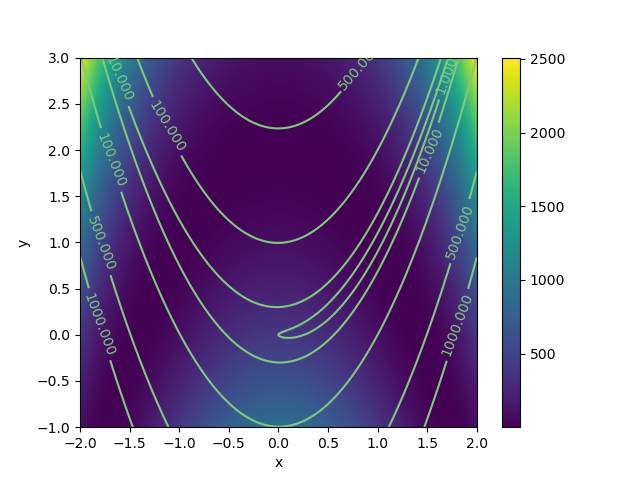
\includegraphics[width=\textwidth]{imgs/plt22}
    \caption{Contour plot}
  \end{subfigure}
  \caption{Rosenbrock Function}
  \label{plt2}
\end{figure}
\subsection{First Derivative}
I find the gradient by applying the chain rule:
\[
\nabla f(x,y) = 
\begin{bmatrix}
    -400x(x_2 - x^2) - 2(1-x_1) \\
    200(x_2 - x^2)            \\
\end{bmatrix}
\]
\subsection{Second Derivative}
Then I find the Hessian matrix:
\[
H(x,x_2) = 
\begin{bmatrix}
    1200x^2 - 400x_2 + 2 & -400x_1     \\
    -400x_1 & 200
\end{bmatrix}
\]

\subsection{Finding a Minimizer}
I can then solve a system of equations in order to find the stationary points:
\begin{align*}
\begin{bmatrix}
    -400x_1(x_2 - x^2) - 2(1-x_1) \\
    200(x_2 - x_1^2)            \\
\end{bmatrix}
&=
\begin{bmatrix}
    0 \\
    0    
\end{bmatrix}\\
\begin{bmatrix}
    x_1 \\
    x_2 \\
\end{bmatrix}
&=
\begin{bmatrix}
    1 \\
    1 \\
\end{bmatrix}
\end{align*}
The system of equations has only one solution, hence $(1,1)^T$ is the only
stationary point. I then determine the type of the stationary point by 
finding the determinant of the hessian matrix:

\[
det(H(1,1)) = 
det\left(\begin{bmatrix}
    1200 - 400 + 2 & -400     \\
    -400 & 200
\end{bmatrix}\right)
= 400 > 0
\]
Since $\frac{df}{dx_1dx_2} = 802 > 0$ and the determinant is positive, I conclude that
$H(1,1)$ is positive definite, and $(1,1)^T$ is the only local minimizer of the
2D Rosenbrock function.

\section{Log-Ellipsoid Function}
\label{sec:log-ellipsoid}

\section{Attractive Sector Functions}
\label{sec:attractive}

\subsection{Overflow in the exponential}
I will prove that following property holds using proof by case:
\[
\log (1+\exp (x))=\log (1+\exp (-|x|))+\max (x, 0)
\]
There are two cases:
\begin{itemize}
\item $x \leq 0$. This case is trivial
  \begin{align*}
    \log (1+\exp (-|x|))+\max (x, 0) &= \log (1+\exp (x)) + 0\\
    &= \log (1+\exp(x))
  \end{align*}
\item $x > 0$
  \begin{align*}
    \log (1+\exp (-|x|))+\max (x, 0) &= \log (1+\exp (-x)) + x\\
    &=\log \left(1 + \frac{1}{e^{x}}\right) + x\\
    &=\log \left(\frac{1 + e^{x}}{e^{x}}\right) + x\\
    &=\log (1 + e^{x}) - \log \left(e^{x}\right) + x\\
    &=\log (1 + e^{x})
  \end{align*}
\end{itemize}
\QEDA\\\\
This formulation is beneficial in a context of a computer implementation, since
when $x$ is a large number, such as $10^8$ in the Attractive-Sector function.
The value of $e^{x}$ would be a huge number that is much larger than
$10^{32}$ or even $10^{64}$. Therefore, it can not fit in any type of CPU
registers and would result in a overflow. $-|x| > 0$ for all real values of $x$,
hence $e^{-|x|}$ would become a very small number for high values of $x$ and
would be rounded to zero, which would eliminate the overflow problem.


%% \begin{figure}
%%   \centering
%%     \centering
%%     \includegraphics[scale=1]{code/plt_p21}
%%   \caption{Plot for the generated dataset}
%%   \label{plt_p21}
%% \end{figure}

%% \begin{lstlisting}[caption="Calculation of g"]
%% def calc_g(Xs, y, w):
%%     N = np.shape(Xs)[0]
%%     # use matrix X of xs instead of for-loop = much faster
%%     X = np.c_[Xs, np.ones(N)]
%%     num = y.T * X
%%     denum = 1 + np.exp(y * (w @ X.T))
%%     M = num.T/denum
%%     # return mean of each row
%%     return (-1 * np.mean(M, axis=1))
%% \end{lstlisting}


%% \begin{figure}
%%   \centering
%%   \begin{subfigure}[b]{\textwidth}
%%     \centering
%%     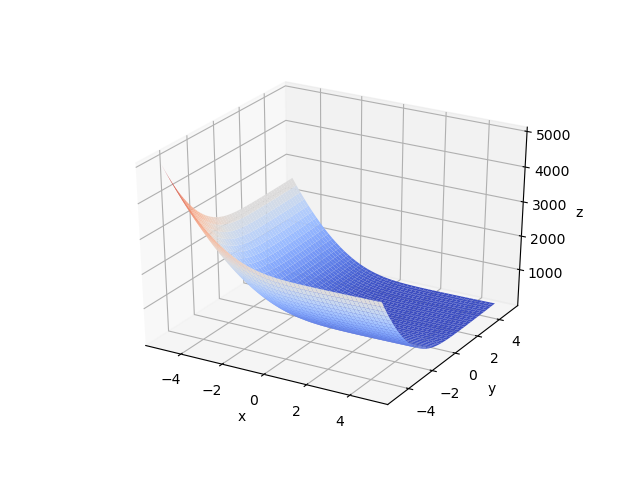
\includegraphics[scale=0.8]{handin/plt51}
%%     \caption{Classification of the training set}
%%   \end{subfigure}
%%   \begin{subfigure}[b]{\textwidth}
%%     \centering
%%     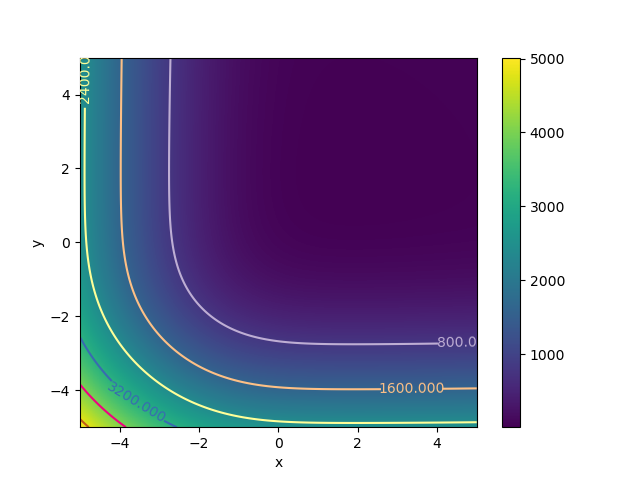
\includegraphics[scale=0.8]{handin/plt52}
%%     \caption{Classification of the test set}
%%   \end{subfigure}
%%   \caption{Exercise 5: Logistic Regression Applied to the Datasets}
%%   \label{plt5}
%% \end{figure}

\end{document}

